\section{Normalization} \label{cha:Problem_Normalization}
In many cases it is advantageous to work with \gls{normalized} problems, i.e., problems with dimensionless variables. In our
case consider again \cref{prb:Non_Normalized_Problem} and replace independent variable $z$ by its normalized counterpart
$x = \frac{z}{L}$. Thus
\begin{subequations} \label{eqn:Normal_Variable}
	\begin{align}
	x & = \frac{1}{L} z \Longleftrightarrow z = \gls{L} \gls{x},  \label{eqn:Normal_New_To_Old} \\
	\frac{d \gls{x}}{d \gls{z}} & = \frac{1}{\gls{L}}, \label{eqn:Normal_Derivative} \\
	\frac{d}{dz} & = \frac{d}{dx} \frac{d \gls{x}}{dz} = \frac{1}{\gls{L}} \frac{d}{dx}. \label{eqn:Normal_Derivative_Total}
	\end{align}
\end{subequations}
Using \crefrange{eqn:Normal_New_To_Old}{eqn:Normal_Derivative_Total} rewrite
\crefrange{eqn:Non_Normalized_Diff_Eq}{eqn:Non_Normalized_Normal_Cond} as
\begin{equation*}
	-\frac{d}{dz} \biggl[ \gls{qBar} \frac{d \overline{u}}{dz} \biggr] =
		-\frac{1}{L} \frac{d}{dx} \biggl[ \glsentryname{qBarLx} \frac{1}{L} \frac{d \overline{u}}{dx} \biggr].
\end{equation*}
Thus
\begin{subequations}	
	\begin{equation}	\label{eqn:Temp_Diff_Eq}
		-\frac{d}{dz} \biggl[ \gls{qBar} \frac{d \overline{u}}{dz} \biggr] =
			\overline{f} \left( Lx \right).
	\end{equation}
	with boundary conditions
	\begin{align}
		\gls{uBar} \Big \vert_{\gls{z} = 0} &= \overline{u} \left( Lx \right) \Big \vert_{x = 0} = \gls{deltaBar},
		\label{eqn:Temp_Dirichlet} \\
		\left[ \gls{qBar} \frac{d \overline{u}}{dz}\right] _{z = L} & =
		\left[ \glsentryname{qBarLx} \frac{1}{L} \frac{d \overline{u} }{ dx } \right]_{x = 1} = \gls{PBar}.
		\label{eqn:Temp_Normal_Cond}
	\end{align}
\end{subequations}	\\
Multiplying \crefrange{eqn:Temp_Diff_Eq}{eqn:Temp_Normal_Cond} by $\frac{ L^2 }{ \glsentryname{qBarX0} }$,
$\frac{ 1 }{ L }$ and $\frac{ L }{ \glsentryname{qBarX0} }$, give
\begin{subequations}
	\begin{align}
		- \frac{ d }{ dx } \Biggl[ \frac{ \glsentryname{qBarLx} }{ \glsentryname{qBarX0} } \frac{ d \overline{u} }{ dx } \Biggr] &
		= \frac{ L^2 \overline{f} \left( Lx \right) }{ \glsentryname{qBarX0} },  \\
		\frac{ 1 }{ L } \overline{u} \left( Lx \right) \Big \vert_{\gls{x} = 0} & = \frac{1}{\gls{L}}  \gls{deltaBar}, \\
		\Biggl[ \frac{ \glssymbol{qBar} \left( Lx \right) }{ \glsentryname{qBarX0} } \frac{d \overline{u}}{dx} \Biggr]_{x = 1}
			&= \frac{ L \gls{PBar} }{ \glsentryname{qBarX0} }.
	\end{align}
\end{subequations}
Now introduce following dimensionless variables and parameters
\begin{subequations}	\label{eqn:Dim_Less_Vars_And_Params}
	{\allowdisplaybreaks
	\begin{align}
		x &= \frac{1}{L} z \label{eqn:Dim_Less_Independent},	\\
		\gls{u} &= \frac{1}{L} \overline{u} \left( Lx \right), \label{eqn:Dim_Less_Solution}	\\
		\glsentryname{uPrime} &= \frac{d\overline{u}}{dx},	\\
		\gls{f} &= \frac{ L^2 \overline{f} \left( Lx \right) }{ \glsentryname{qBarX0} },	\label{eqn:Dim_Less_Load} \\
		\gls{q} &= \frac{ \glsentryname{qBarLx} }{ \glsentryname{qBarX0} },	\label{eqn:Dim_Less_q}	\\
		\gls{delta} &= \frac{1}{L} \gls{deltaBar},	\label{eqn:Dim_Less_Delta} \\
		\gls{P} &= \frac{ L \gls{PBar} }{ \glsentryname{qBarX0} }.	\label{eqn:Dim_Less_P}
	\end{align}}	% end of \allowdisplaybreaks
\end{subequations}
\Cref{prb:Normalized_Problem} below is a normalized \gls{BVP} and the dimensionless version of
\cref{prb:Non_Normalized_Problem} in terms of variables in \crefrange{eqn:Dim_Less_Independent}{eqn:Dim_Less_P}. In the remaining
of this document we will focus on this problem, see \cref{fig:Problem_Normalized}.
\begin{figure}
	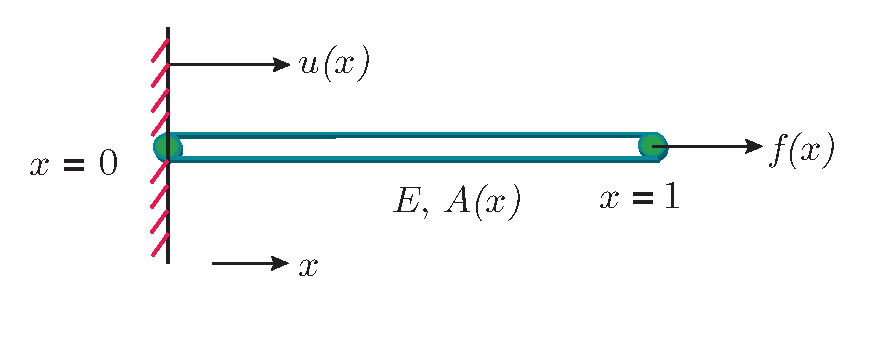
\includegraphics[width = \textwidth]{../figures/problem-normalized}
	\caption[The Normalized Bar Problem]
	{The Normalized Bar Problem}
	\label{fig:Problem_Normalized}
\end{figure}

\begin{problem} \label{prb:Normalized_Problem}
	Governing equation for the \gls{bar}'s displacement function is
	\begin{subequations} \label{eqn:Normalized_Problem}
		\begin{equation}	\label{eqn:Normalized_Diff_Eq}
			-\frac{d}{dx} \biggl[ \gls{q} \glsentryname{uPrime} \biggr] = \gls{f},
			\quad x \in \left( 0, 1 \right),
		\end{equation}
		with boundary conditions
		\begin{align}
			\gls{u} \bigg \vert_{x = 0} &= \gls{delta},  \label{eqn:Normalized_Dirichlet_Cond}  \\
			\biggl[ q \left( x \right) \frac{du}{dx} \biggr]_{x = 1} &= P, \label{eqn:Normalized_Normal_Cond}
		\end{align}
		where dimensionless variables and parameters $x$, $u \left( x \right)$, $f \left( x \right)$, $q \left( x \right)$,
		$\gls{delta}$ and $P$ are given in \crefrange{eqn:Dim_Less_Independent}{eqn:Dim_Less_P}.
	\end{subequations}
\end{problem}
%